\chapter{Results} \label{chap:res}

\section{Analysis of Olympic Games Duration and Evolution}

The Gantt chart in Figure \ref{fig:gantt_olympics} illustrates the scheduling and duration of both Summer and Winter Olympic Games from the inaugural Athens Games in 1896 to the events in 2022. It highlights key milestones and trends in the evolution of the Olympics.

\begin{figure}[ht]
    \centering
    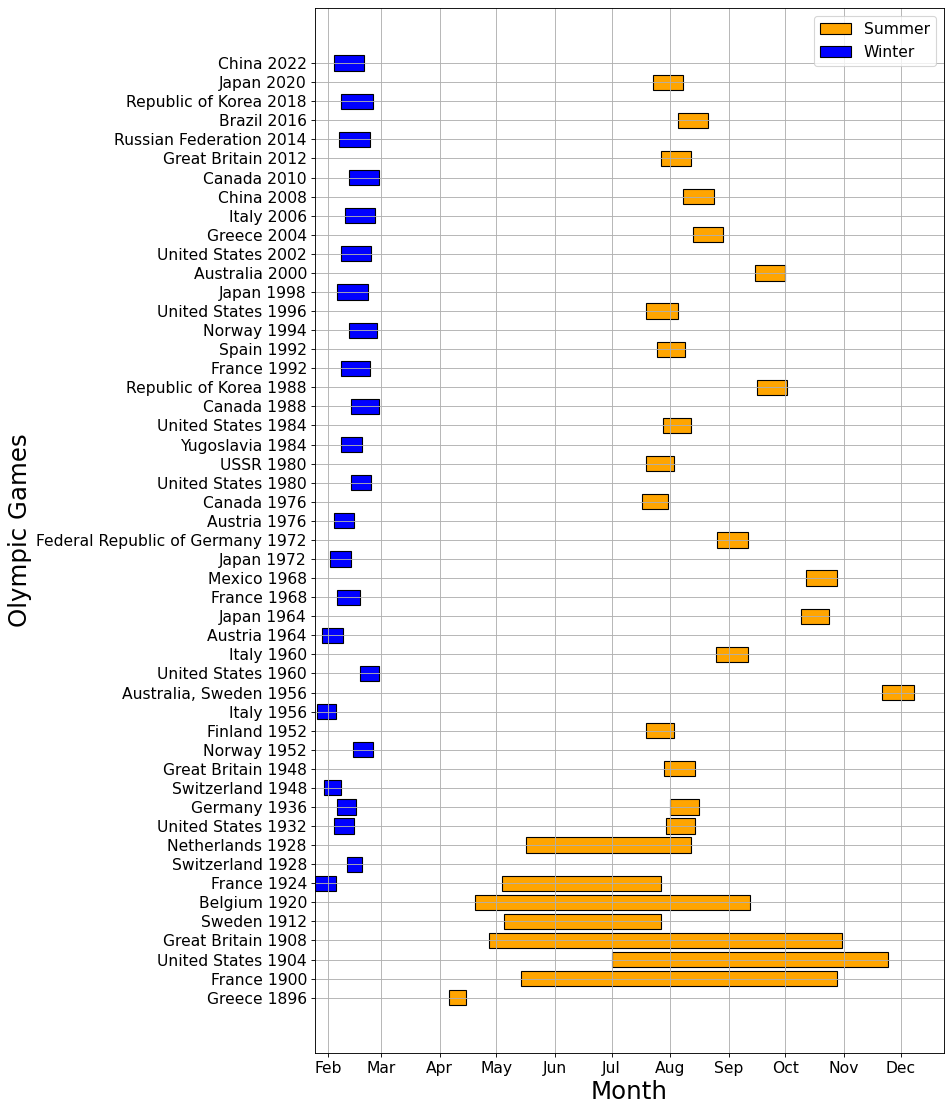
\includegraphics[width=0.8\textwidth]{Gantt Chart of Olympic Games.png}
    \caption{Gantt Chart of Olympic Games Duration}
    \label{fig:gantt_olympics}
\end{figure}

The modern Olympics began in 1896 with exclusively male participants and a limited schedule of events lasting 10 days. By 1900, the Paris Games introduced women's participation and expanded the schedule to over five months, integrating the Olympics into the World’s Fair. This unusual duration reflected the scattered organization and the addition of new sports like golf, tennis, and rowing. Over time, the duration became more standardized, with events typically lasting around two weeks by the mid-20th century, reflecting the Games' growing scale and complexity.

The Winter Olympics were introduced in Chamonix, France, in 1924, marking the start of a separate seasonal competition for winter sports. Notably, France hosted both the Summer and Winter Games in the same year, solidifying its pivotal role in Olympic history.

Additionally, the chart captures regular scheduling patterns, with Summer Games typically held between July and August and Winter Games in February. It also reveals disruptions caused by global conflicts, including cancellations during World War I and World War II.

\section{Chord Diagram for Migration Flow}

Given the increasing rate of immigration over the past few decades, we decided to analyze immigration in the context of the Olympic Games, specifically focusing on Olympic athletes who represent countries different from the ones in which they were born. A key component for this analysis was the inclusion of athletes' birth countries, which were not initially present in the dataset. To address this, we used web scraping to extract athletes' birth countries from their Wikipedia pages and added this information as a new feature to the dataset. Since there have been significant changes in the names and territories of countries over time, we decided to focus only on the last 10 Olympic Games to ensure consistency.

To visualize this analysis, we used a chord diagram. A chord diagram is a graphical tool designed to show relationships between entities, where the flow of migration is represented by the chords. The source and destination countries of the migration are indicated by the base and arrowhead of each chord, respectively. The width of each arc is proportional to the number of athletes migrating from one country to another.

In our chord diagram, the countries are grouped by sub-continent, with a total of 9 sub-continents, plus the Refugee Olympic Team, which is treated as a separate category. Each sub-continent is assigned a unique color theme to improve the clarity of the visualization. To make the analysis more manageable and focused, we only included countries with more than 10 immigrant athletes in the diagram. This filter ensures that the visualization highlights significant migration flows.

\begin{figure}[ht]
    \centering
    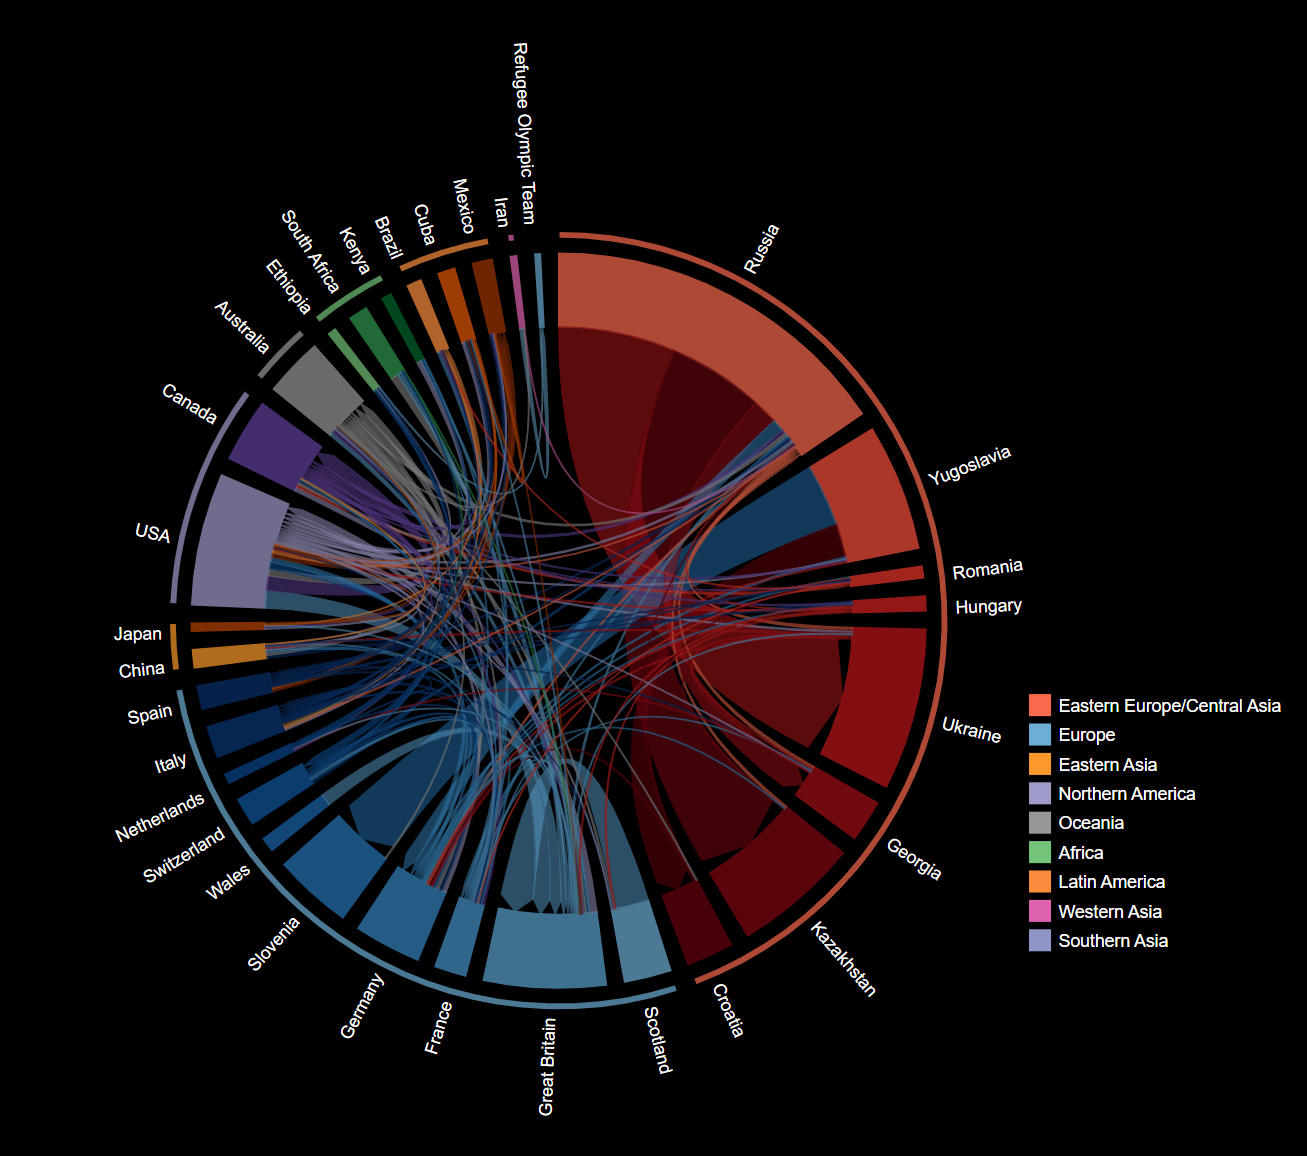
\includegraphics[width=0.8\textwidth]{chord_diagram.png}
    \caption{Chord Diagram: Visualizing Olympic Athletes' Migration Flows Since 2010}
    \label{fig:choropleth_map}
\end{figure}

\subsection{Features of the Diagram}
An interactive feature of this diagram is that when hovering over a country's name, additional information is displayed, including the total number of incoming and outgoing immigrants for that country. Additionally, when hovering over a country, the opacity of arrows that do not originate from or end in that country is reduced. This allows the user to focus on immigration flows specifically related to the selected country, highlighting it as the source or destination
\subsection{Insights from the Diagram}
The diagram provides valuable insights into immigration patterns. Most visible immigration flows align closely with political and geographical changes in the world. In particular, highly developed countries like the United States and Britain emerge as major destinations for immigrants, likely due to the better opportunities and higher quality of life they offer.

However, the diagram also reveals patterns specific to the unique nature of the dataset. For instance, Russia was banned from participating in the 2016 Rio and 2020 Tokyo Olympics due to doping violations. In such cases, many Russian athletes opted to compete under other countries' flags just to continue participating in the games.

Another intriguing trend is the movement of athletes between countries in pursuit of better athletic opportunities. For example, some U.S. athletes appear to have moved to Latin American countries, possibly because it was easier to qualify for the Olympic team there. 


\section{Dynamic Choropleths and Bubble Maps}

The dynamic choropleth and bubble maps were designed to provide an interactive exploration of Olympic trends worldwide. These maps enable users to visualize data such as the frequency of Olympic hosting by country, the number of athlete debuts, and medal counts. With dynamic filtering options and multiple visualization styles, they offer a versatile and engaging way to analyze key aspects of Olympic history.

The choropleth map excels at conveying spatial patterns and regional comparisons through color intensity, making it ideal for quickly identifying geographical trends. However, it may obscure information for smaller countries due to their limited map space. In contrast, the bubble map highlights individual data points with proportional circle sizes, ensuring that smaller countries remain visible and providing a more precise representation of numerical values. On the downside, bubble maps can become cluttered in regions with dense data points, potentially making it harder to interpret overlapping bubbles. Together, these visualization styles complement each other, balancing clarity and detail depending on the user's analytical needs.

\begin{figure}[ht]
    \centering
    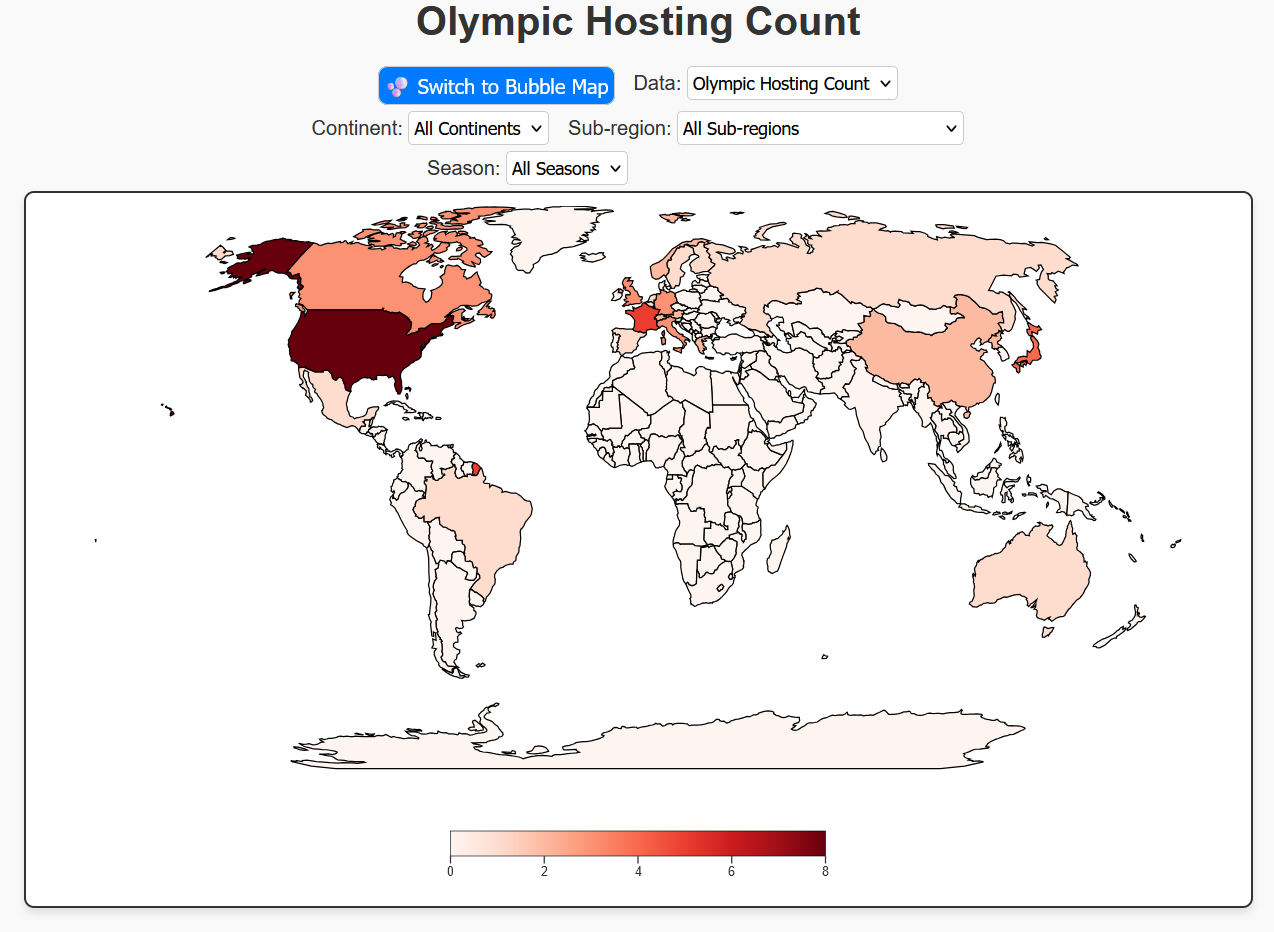
\includegraphics[width=0.8\textwidth]{Dynamic Choropleth.png}
    \caption{Dynamic Choropleth Map: Visualizing Olympic Hosting Trends}
    \label{fig:choropleth_map}
\end{figure}

\begin{figure}[ht]
    \centering
    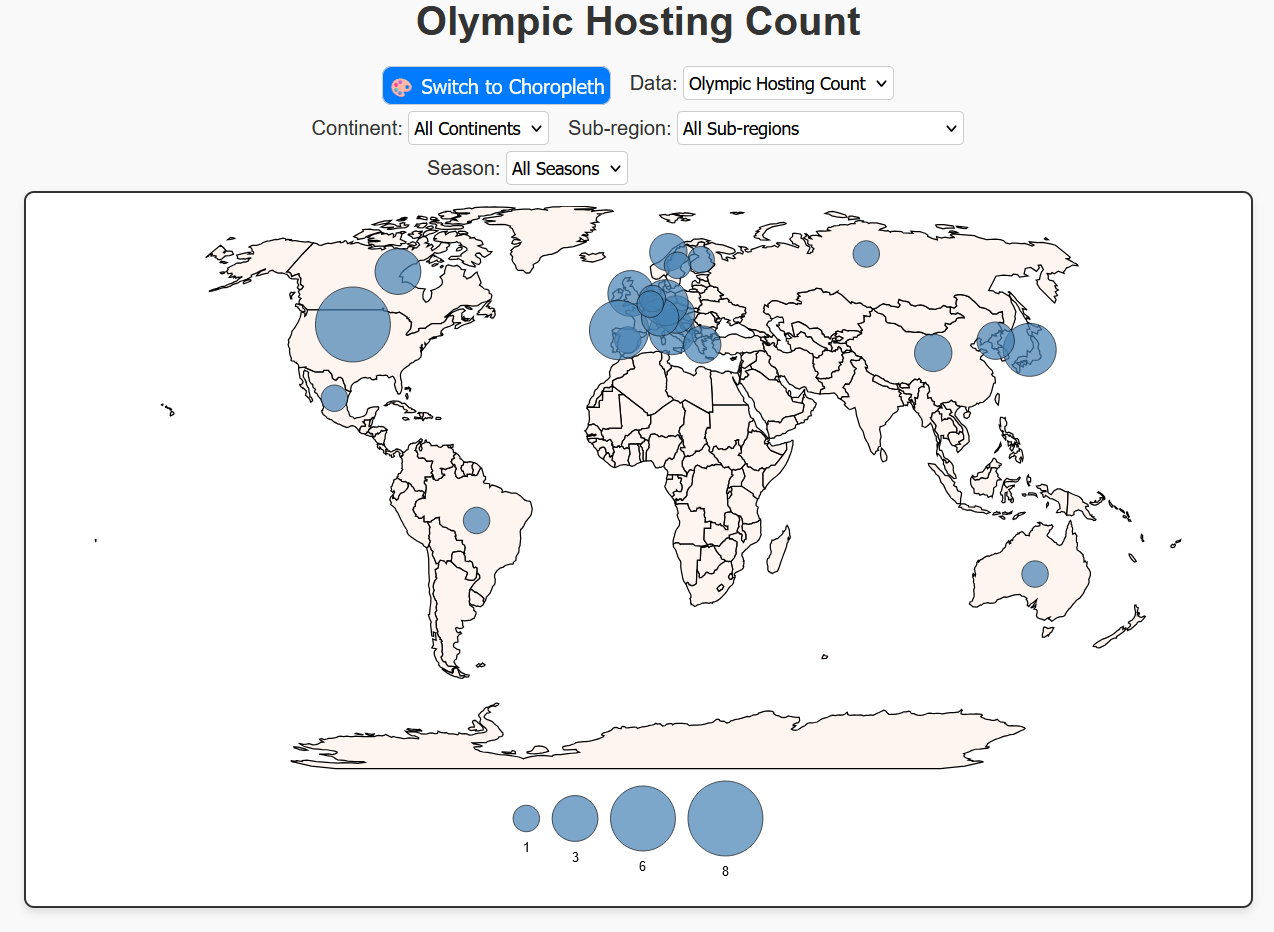
\includegraphics[width=0.8\textwidth]{Dynamic Bubble Map.png}
    \caption{Dynamic Bubble Map: Visualizing Olympic Hosting Trends}
    \label{fig:bubble_map}
\end{figure}

\subsection{Features of the Maps}

The maps provide the following functionalities:
\begin{itemize}
    \item \textbf{Visualization Modes:} Users can switch between a choropleth map (Figure \ref{fig:choropleth_map}) and a bubble map (Figure \ref{fig:bubble_map}) for different visual representations of hosting frequency.
    \item \textbf{Filters and Options:} Filtering options include continents, sub-regions, seasons (Summer or Winter), medal types (Gold, Silver or Bronze), if applicable. These allow users to customize the view and focus on specific geographic or temporal trends.
    \item \textbf{Interactivity:} Both maps feature hover-over tooltips displaying detailed information, such as the number of times a country has hosted the Olympics.
\end{itemize}

\subsection{Insights from the Maps}

These maps reveal several insights into Olympic hosting trends:
\begin{itemize}
    \item Countries such as the United States, Great Britain, and France stand out in number of debuts and high hosting frequencies, reflecting their longstanding involvement in the Olympics.
    \item Hosting occurrences are concentrated in Europe and North America, particularly during the early years of the modern Olympics.
    \item The inclusion of filtering options enables the identification of hosting trends by region, season, and medal type, highlighting the geographical expansion of the Games over time.
\end{itemize}

The combination of choropleth and bubble maps exemplifies the power of interactive visualizations, enabling a flexible exploration of the data while revealing key trends and disparities in Olympic hosting.

\section{Olympic Rivalries Network Visualization}

In addition to the previously discussed analyses, we developed an interactive visualization that highlights the rivalry patterns in the Olympic Games. This \textbf{Olympic Rivalries Network} provides an engaging way to explore competitive relationships among countries based on their historical medal tallies and rivalry strength.

\begin{figure}[ht]
    \centering
    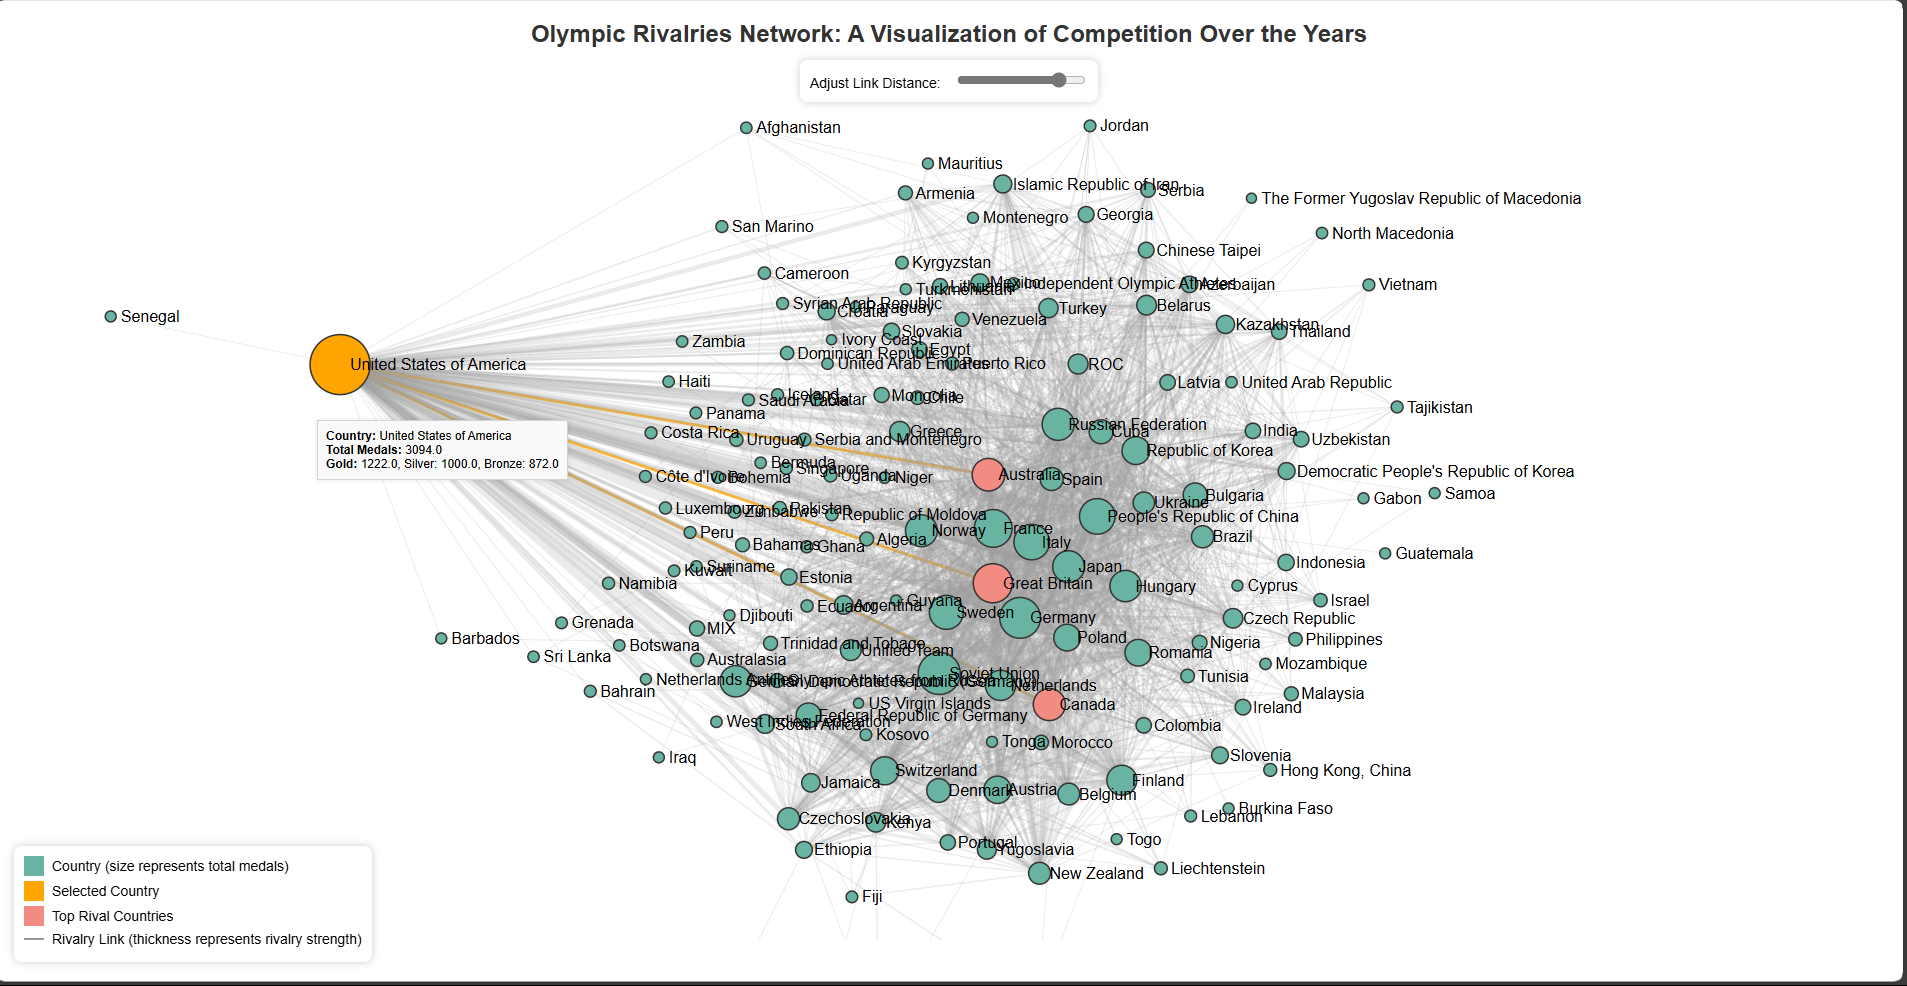
\includegraphics[width=0.8\textwidth]{olympic_rivalries_network.png}
    \caption{Olympic Rivalries Network Visualization}
    \label{fig:olympic_rivalries_network}
\end{figure}

\subsection{Features of the Visualization}
The Olympic Rivalries Network is an interactive graph-based visualization where:
\begin{itemize}
    \item \textbf{Nodes represent countries}, and their size is proportional to the total number of medals won by each country.
    \item \textbf{Edges (links) represent rivalry strength}, with thickness proportional to the intensity of the rivalry (determined by shared events, medal contention, and other metrics).
    \item Users can hover over nodes to view detailed information, including:
    \begin{itemize}
        \item Total medals, broken down by Gold, Silver, and Bronze.
        \item The top rival countries for the selected country.
    \end{itemize}
    \item Clicking on a node highlights the top three rival countries for the selected country, while emphasizing the edges connecting them.
    \item A legend, positioned at the bottom-left corner, explains the color-coding and node/edge properties.
    \item A slider allows users to dynamically adjust the "link distance" (spacing between nodes), facilitating better exploration of densely connected regions of the graph.
\end{itemize}

\subsection{Insights from the Visualization}
\begin{itemize}
    \item \textbf{Historical Rivalries:} The network effectively captures iconic rivalries, such as the competitive dominance between the United States and the Soviet Union during the Cold War era.
    \item \textbf{Emerging Rivalries:} The visualization also highlights emerging rivalries, such as those between countries in rapidly growing sporting regions like Asia and South America.
    \item \textbf{Team Size and Medal Dominance:} The size of the nodes reflects the sporting dominance of traditional powerhouses like the United States and China, which have large medal counts and broader participation.
\end{itemize}

This network visualization complements other data representations by focusing on relationships and rivalries, offering a unique lens through which to understand the Olympic Games' competitive dynamics. The combination of interactivity, visual clarity, and comprehensive information enhances both engagement and analytical depth for users.

\section{Cumulative Olympic Medals Visualization}

To explore the progression of Olympic success over time, we developed an interactive visualization focusing on the cumulative medal counts for the top-performing countries in Olympic history. This visualization allows users to analyze trends, compare countries, and observe how nations have evolved in their athletic achievements since the inception of the modern Olympics in 1896.

\begin{figure}[ht]
    \centering
    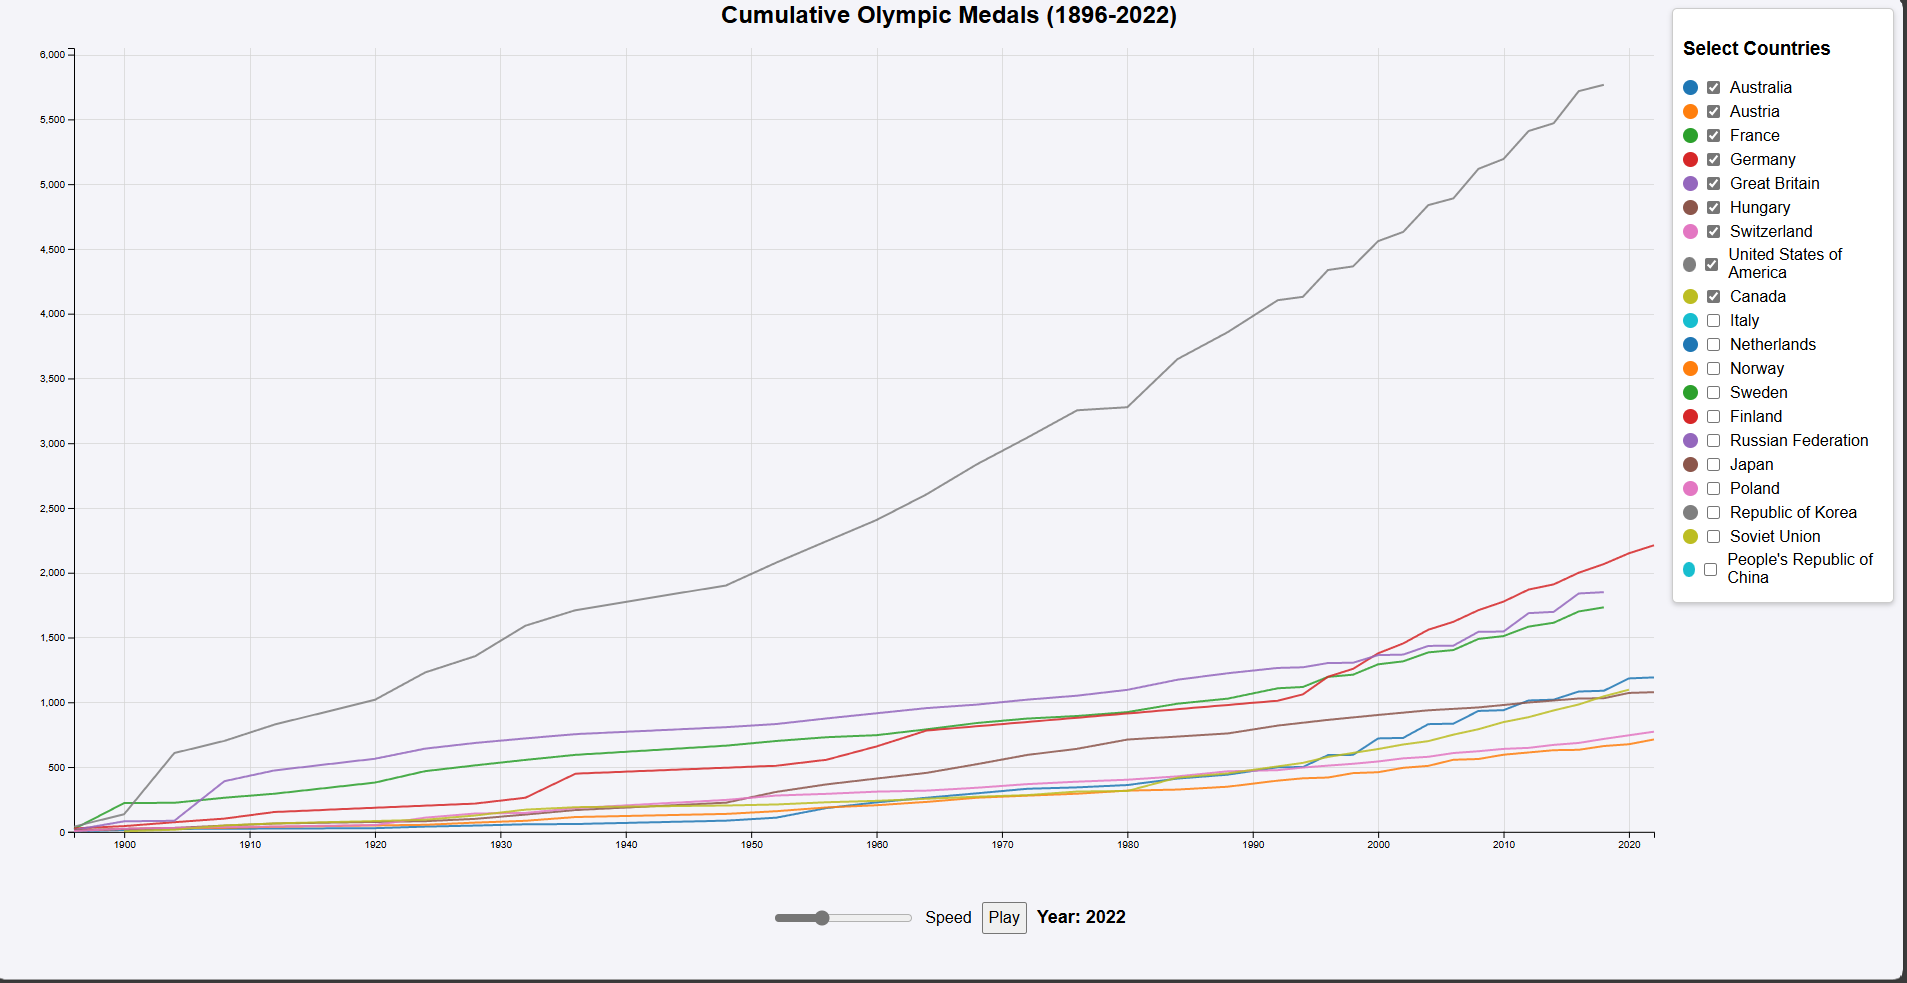
\includegraphics[width=0.8\textwidth]{cumulative_olympic_medals.png}
    \caption{Cumulative Olympic Medals Visualization (1896-2022)}
    \label{fig:cumulative_medals}
\end{figure}

\subsection{Features of the Visualization}
The Cumulative Olympic Medals Visualization includes the following features:
\begin{itemize}
    \item \textbf{Top 20 Medal-Winning Countries:} The visualization focuses on the top 20 countries with the highest total medal counts to provide a clear and meaningful analysis of Olympic trends.
    \item \textbf{Dynamic Country Selection:} Users can select or deselect countries of interest using a side panel. Each country is represented by a unique color, and a color legend is displayed for quick reference.
    \item \textbf{Animated Evolution:} Once countries are selected, the evolution of their cumulative medal counts is shown as an animated line chart. The animation ensures a smooth, continuous progression, emphasizing yearly trends and major leaps in medal counts.
    \item \textbf{Adjustable Speed:} A speed slider enables users to control the animation speed, accommodating different viewing preferences and levels of detail.
    \item \textbf{Interactive Year Display:} The current year is dynamically displayed during the animation, helping users correlate medal counts with specific Olympic Games.
    \item \textbf{Gridlines and Axes:} Gridlines provide context for the data points, and clearly labeled axes highlight the timeline and medal counts for better interpretability.
\end{itemize}

\subsection{Insights from the Visualization}
This visualization provides several insights into Olympic medal trends:
\begin{itemize}
    \item \textbf{Historical Dominance:} Countries like the United States and the Soviet Union demonstrate significant cumulative medal counts, reflecting their longstanding dominance in the Olympics.
    \item \textbf{Emerging Powerhouses:} Nations such as China show sharp increases in medal counts, particularly after their economic and athletic investments in the late 20th century.
    \item \textbf{Impact of Historical Events:} Global conflicts, such as the World Wars, and boycotts are evident in the periods of slower growth for certain countries.
    \item \textbf{Comparative Analysis:} By visualizing multiple countries simultaneously, users can identify gaps and overlaps in medal-winning trajectories.
\end{itemize}

\section{Olympic Participation Trends Over Time Visualization}

To analyze the growth and changes in participation over the history of the Olympic Games, we developed a visualization that tracks the number of participating countries over time. This visualization provides a clear depiction of historical patterns, interruptions, and milestones in Olympic history.

\begin{figure}[ht]
    \centering
    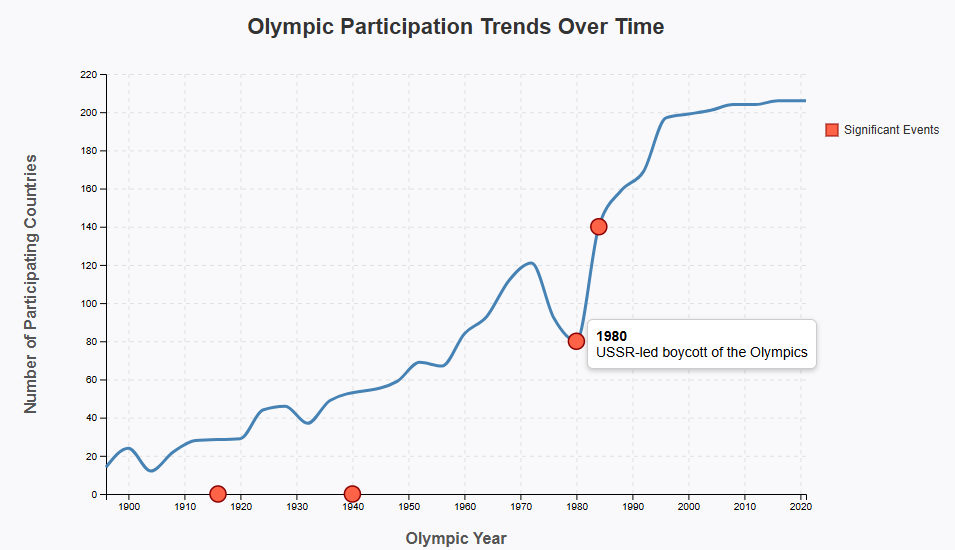
\includegraphics[width=0.8\textwidth]{olympic_participation_trends.png}
    \caption{Olympic Participation Trends Over Time (1896-2022)}
    \label{fig:participation_trends}
\end{figure}

\subsection{Features of the Visualization}
The Olympic Participation Trends visualization includes the following features:
\begin{itemize}
    \item \textbf{Line Chart with Gridlines:} A line chart is used to represent the number of participating countries over time, with gridlines providing context for interpreting the data.
    \item \textbf{Significant Events Marked:} Key events, such as interruptions due to global conflicts and political boycotts, are marked with red circles on the line chart. These markers align with the participation trend, ensuring clarity and relevance.
    \item \textbf{Interactive Tooltips:} Hovering over the event markers displays additional information about the event, including its year and description, providing context for notable changes in participation.
    \item \textbf{Axes with Descriptive Labels:} The x-axis represents the Olympic years, and the y-axis indicates the number of participating countries, with clear labels for improved readability.
    \item \textbf{Legend for Event Markers:} A legend is included to clarify the meaning of the red event markers, ensuring that users understand their significance.
\end{itemize}

\subsection{Insights from the Visualization}
This visualization highlights several important insights:
\begin{itemize}
    \item \textbf{Growth in Participation:} The number of participating countries has grown steadily over time, reflecting the globalization of the Olympics.
    \item \textbf{Impact of Global Events:} Major disruptions, such as World Wars and political boycotts, are clearly visible in the trends, illustrating how external factors have influenced Olympic participation.
    \item \textbf{Milestones in Olympic History:} Key moments, such as the inclusion of more countries in the mid-20th century, underscore the expansion and inclusivity of the Olympic Games.
\end{itemize}

This visualization effectively combines historical data with interactive elements to provide a comprehensive view of Olympic participation trends. By emphasizing significant events and enabling user interaction, it enhances the exploration and understanding of Olympic history.

\section{Olympic Medal Density Map Over Time}

To visualize the geographical distribution of Olympic medals over time, we created an interactive density map. This visualization showcases the number of medals won by each country in a given year, enabling a clear understanding of regional dominance and trends throughout Olympic history.

\begin{figure}[ht]
    \centering
    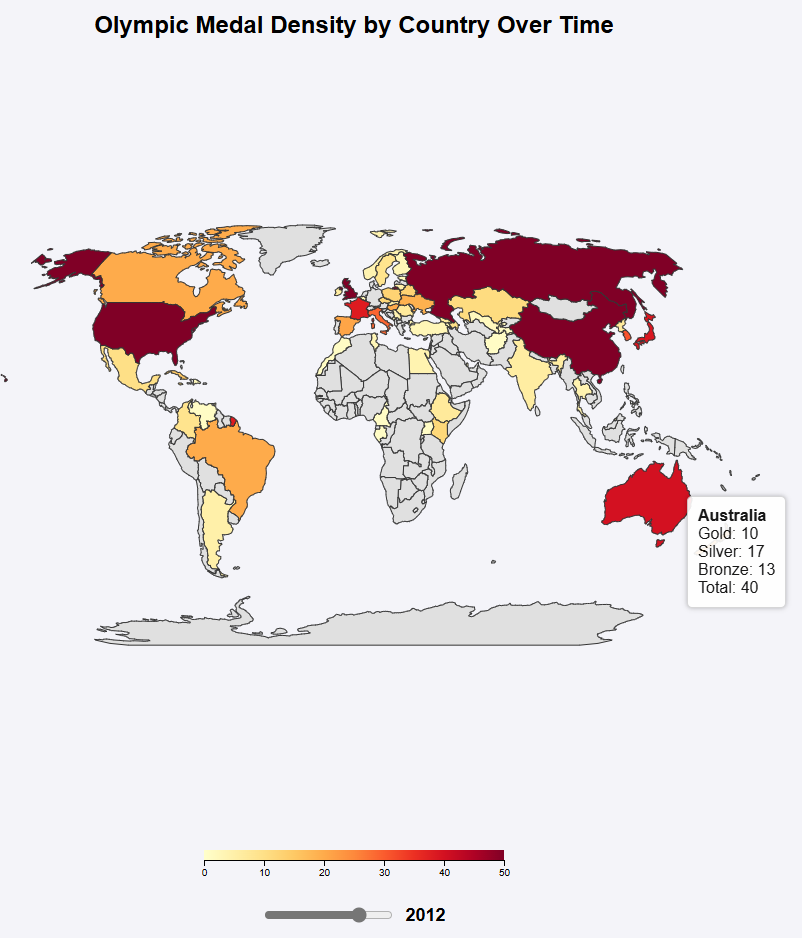
\includegraphics[width=0.8\textwidth]{olympic_medal_density_map.png}
    \caption{Olympic Medal Density Map by Country Over Time}
    \label{fig:medal_density_map}
\end{figure}

\subsection{Features of the Visualization}
The Olympic Medal Density Map includes the following features:
\begin{itemize}
    \item \textbf{Interactive World Map:} Countries are shaded based on the total number of medals won in a given year. A sequential color scale, ranging from light yellow to deep red, represents medal counts, with darker colors indicating higher totals.
    \item \textbf{Dynamic Year Slider:} Users can explore medal densities across years by adjusting a slider. The map updates dynamically to reflect the chosen year.
    \item \textbf{Tooltip Information:} Hovering over a country displays detailed medal information, including counts of gold, silver, and bronze medals, along with the total medals won for the selected year.
    \item \textbf{Color Legend:} A gradient color bar at the bottom provides context for interpreting the medal density, with clear labels indicating the range of medal counts.
\end{itemize}

\subsection{Insights from the Visualization}
This map reveals several key insights into the geographical distribution of Olympic success:
\begin{itemize}
    \item \textbf{Regional Dominance:} Developed countries, including the United States, Russia, and China, consistently dominate the medal counts, reflecting their strong sports programs and infrastructure.
    \item \textbf{Emerging Nations:} Over time, the visualization highlights the increasing presence of emerging nations on the Olympic stage, particularly from Africa, Asia, and South America.
    \item \textbf{Historical Context:} The map effectively visualizes disruptions caused by historical events. For example, during years of political boycotts or global conflicts, certain countries are notably absent from the medal tally.
    \item \textbf{Performance Evolution:} Users can observe trends in a country's medal performance over time, offering insights into periods of peak success or decline.
\end{itemize}

\section{Data Dashboard}
This HTML page serves as a centralized hub for all visualizations, consolidating plots and charts to offer a clear and organized view of the data. Each plot acts as a clickable link, redirecting users to the corresponding full visualization page. A description overlay appears on hover, providing additional context for each plot.

The page leverages various HTML and CSS features, including iframe for embedding visualizations, zoom and transform for dynamic scaling, and hover effects for interactivity. Additionally, the responsive grid layout ensures the visualizations adapt seamlessly to different screen sizes, maintaining proper spacing and alignment for an optimized user experience.

\begin{figure}[ht]
    \centering
    \includegraphics[width=0.8\textwidth]{DataDashbord.png}
    \caption{Data Dashboard: A centralized hub for displaying and accessing all visualizations}
    \label{fig:choropleth_map}
\end{figure}
